By analysing the ``XTrain.json'' feature training set, some important
information can be found. For example, the file contains both the article
headline, and the article link. Training utilising the article link will give
100\% accuracy, as all fake news headlines are sourced from the satirical news
website ``The Onion'', while all real news headlines are sourced from the
``Huffington Post''. As such, models should only be fit using the article
headlines.

\begin{lstlisting}[language=Python, caption={``countTopWords'' Function},
label={lst:cntTopWords}]
def countTopWords(featureTrainCounts, count_vect, n):
    sum_words = featureTrainCounts.sum(axis=0)
    words_freq = [(word, sum_words[0, idx])
                  for word, idx in count_vect.vocabulary_.items()]
    words_freq = sorted(words_freq, key=lambda x: x[1], reverse=True)
    return words_freq
\end{lstlisting}

In order to count the most frequently occurring words in each feature, the
``countTopWords'' function is used. This function, as in Listing
\ref{lst:cntTopWords}, takes the matrix output of the ``CountVectorizer''
function, adds the occurrences of each word, and sorts the values into a list of
tuples of word-frequency pairs\cite{boujon_2019}. This list can then be returned
to the calling function.

In order to plot the most frequently occurring words within the training set,
the ``plotBagOfWords'' function is used. This function , as shown in Listing
\ref{lst:plotBOW}, takes a plot title, the
output from the ``countTopWords'' function, and the number of terms, and plots
them in a bar plot of words against frequency. This bar plot is plotted
horizontally for clearer readability.

\begin{lstlisting}[language=Python, caption={``plotBagOfWords'' Function},
label={lst:plotBOW}]
def plotBagOfWords(plotTitle, data, n):
    sns.set(style="darkgrid")
    x = []
    y = []
    for N in range(n):
        x += [data[N][0]]
        y += [data[N][1]]
        print(x)
        print(y)
    ax = sns.barplot(x=y, y=x, color="blue")
    ax.set(xlabel='Frequency', ylabel='Word', title=plotTitle)
    plt.show()
\end{lstlisting}

To test the difference in allowing or removing stop words - presumed
``uninformative'' words\cite{} - the ``bagOfWords'', ``countTopWords'', and
``plotBagOfWords'' functions must be called with the ``stopWords'' parameter set
to ``True'' and ``False''. The following plots show the differences when stop
words are and aren't included.

\begin{figure}[H]
	\centering
	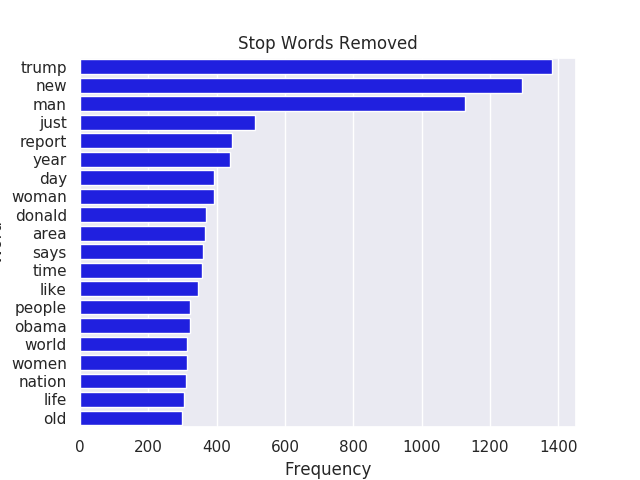
\includegraphics[width=0.8\textwidth]{images/stopWordsRemoved}
	\caption{Most Frequent Terms - Stop Words Removed}
	\label{fig:plotNoStops}
\end{figure}

\begin{figure}[H]
	\centering
	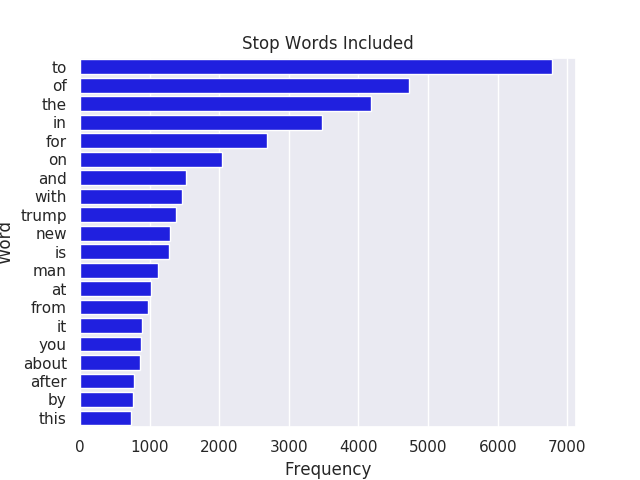
\includegraphics[width=0.8\textwidth]{images/stopWordsIncluded}
	\caption{Most Frequent Terms - Stop Words Included}
	\label{fig:plotStops}
\end{figure}

In order to verify these results, the ``yellowbrick'' library was used to
vizualize the data\cite{tfdYB}. The results from this verification can be seen in Figures
\ref{fig:plotNoStopsYB} and \ref{fig:plotStopsYB}.

\begin{figure}[H]
	\centering
	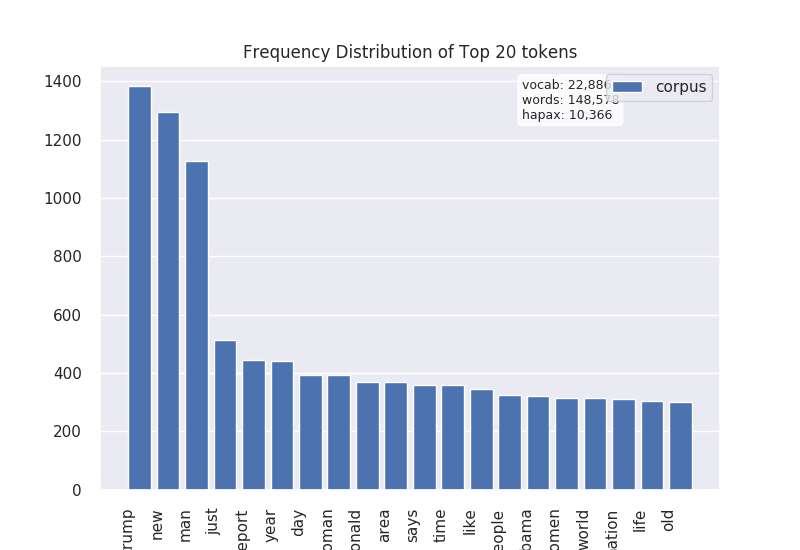
\includegraphics[width=0.8\textwidth]{images/SWRemovedYB}
	\caption{Most Frequent Terms - Stop Words Removed - Yellowbrick}
	\label{fig:plotNoStopsYB}
\end{figure}

\begin{figure}[H]
	\centering
	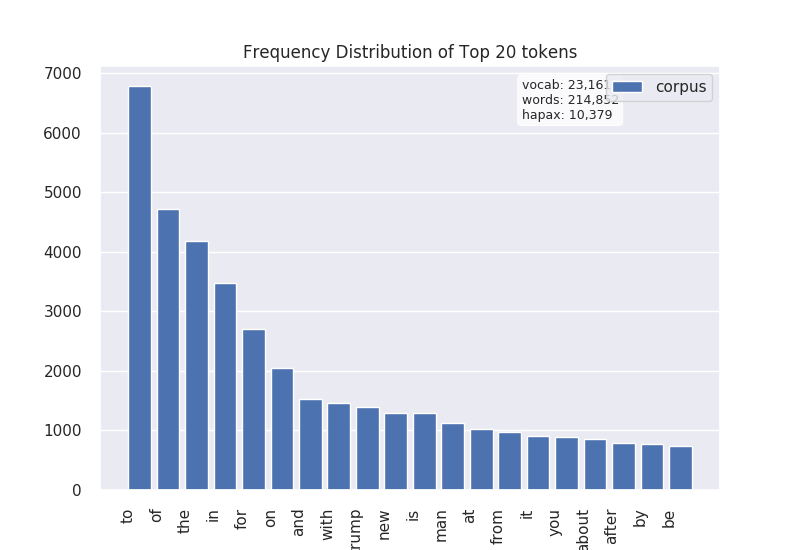
\includegraphics[width=0.8\textwidth]{images/SWIncludedYB}
	\caption{Most Frequent Terms - Stop Words Included - Yellowbrick}
	\label{fig:plotStopsYB}
\end{figure}

As seen in Figure \ref{fig:plotNoStops}, the most frequent word within the
training set, with stop words removed, is ``Trump''. This gives some context to
the nature of the content within the dataset. However, in Figure
\ref{fig:plotStops}, the most frequent word within the training set without
removing stop words is ``to''. This word gives no contextual information, and as
such, shows the benefits of removing stop words within the Bag of Words model.

\begin{lstlisting}[language=Python, caption={``countHeadlineLength'' Function},
label={lst:cntLength}]
def countHeadlineLength(features, target):
    fakeLen = np.array([])
    realLen = np.array([])
    for index, value in target.items():
        # print("Index: {}, Value: {}".format(index, value))
        if(value == 1):
            fakeLen = np.append(fakeLen, len(features.headline.loc[index]))
        else:
            realLen = np.append(realLen, len(features.headline.loc[index]))
        # print(features.headline.loc[index])
    print(np.mean(fakeLen))
    print(np.mean(realLen))
    plotHeadlineLength(fakeLen, realLen)
\end{lstlisting}

\par In addition to the frequency of the words, the length of the headlines can
be assessed. The ``countHeadlineLength'' function, as shown in Listing
\ref{lst:cntLength}, takes the feature and target datasets as inputs, iterates
over the target set, and creates two numpy arrays, one containing the length of
the ``real'' article headlines, and one with the ``fake'' articel headlines. The
mean value of these arrays can then be taken. In order to visualize this
information, two boxplots are drawn, using the seaborn library ``boxplot''
function. The ``plotHeadlineLength'' function takes in the real and fake
headline length arrays are passed in to the function, which converts each to a
pandas DataFrame object in order to plot them.

\begin{lstlisting}[language=Python, caption={``plotHeadlineLength'' Function},
label={lst:plotLength}]
def plotHeadlineLength(fake, real):
    dataFake = pd.DataFrame(fake)
    dataReal = pd.DataFrame(real)
    sns.set(style='darkgrid')
    ax = sns.boxplot(data=dataFake, orient="h")
    ax.set(xlabel='Headline Length', ylabel='', title="Fake Headline Length")
    plt.savefig('fakeHeadlineLength.png')
    plt.show()
    bx = sns.boxplot(data=dataReal, orient="h")
    bx.set(xlabel='Headline Length', ylabel='', title="Real Headline Length")
    plt.savefig('realHeadlineLength.png')
    plt.show()
\end{lstlisting}

The resulting boxplots from Listing \ref{lst:plotLength} for the fake and real
headlines are shown below in Figures \ref{fig:fakeLength}, and
\ref{fig:realLength} respectively.

\begin{figure}[H]
	\centering
	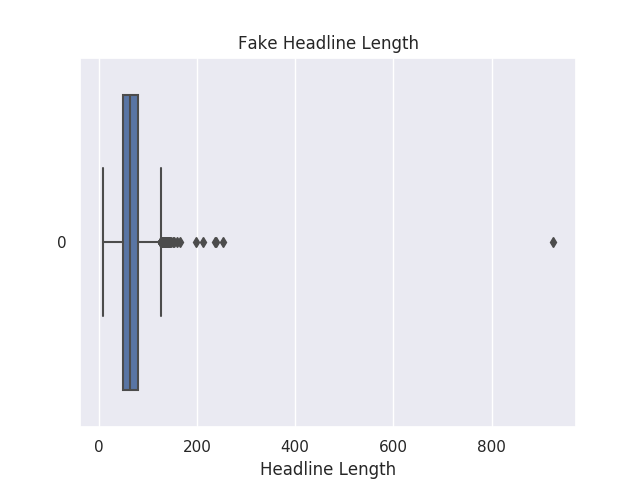
\includegraphics[width=0.8\textwidth]{images/fakeHeadlineLength}
	\caption{Lengths of the ``Fake'' Headlines}
	\label{fig:fakeLength}
\end{figure}

The mean length of a fake headline is approximately 65.48 characters. There is a
maximum length of 926 characters, and a minumum length of 8 characters.

\begin{figure}[H]
	\centering
	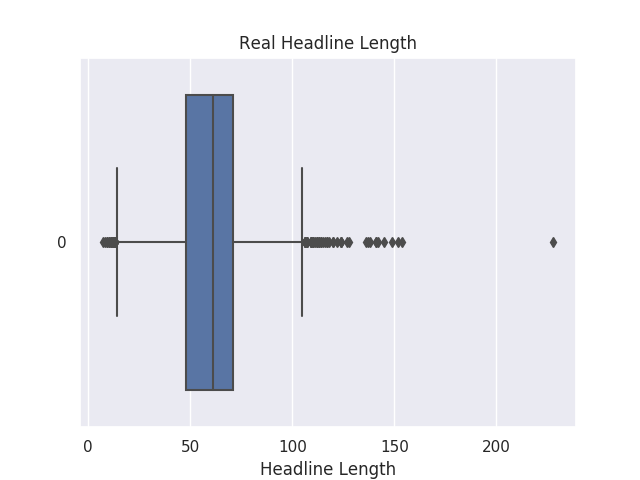
\includegraphics[width=0.8\textwidth]{images/realHeadlineLength}
	\caption{Lengths of the ``Real'' Headlines}
	\label{fig:realLength}
\end{figure}

The mean length of a real headline is approximately 59.46 characters. There is a
maximum length of 228 characters, and a minimum length of 7 characters.

\par From the above analysis it can be seen that the length of headlines for
fake headlines are, on average, longer, with a greater value outlier. As such,
the length of real headlines are shorter, with smaller outlier values.
